\documentclass[12pt]{article}

\usepackage{sbc-template}
\usepackage{float} % Pacote para a opção [H]
\usepackage{graphicx,url}


\usepackage[brazil]{babel}   
\usepackage[utf8]{inputenc}  

     
\sloppy

\title{Artigo de Software Front-end}

\author{Daniella Ferreira Marques}


\address{Instituto Federal do Piauí - IFPI - Campus Picos
\email{isabelmarques902@gmail.com}
}

\begin{document} 

\maketitle

\begin{abstract}
  Tradução do texto original para o inglês.   
  
  \textbf{Keywords:}
\end{abstract}
     
\begin{resumo}
   Para a elaboração do resumo e do abstract em um trabalho acadêmico, é recomendado utilizar fontes como Arial ou Times New Roman, tamanho 12, com espaçamento entre linhas simples de 1,0. É importante que o resumo contenha entre 150 a 250 palavras, incluindo informações sobre os objetivos do estudo, fundamentação teórica, metodologia, resultados e conclusões ou considerações. É fundamental que o texto não contenha citações ou siglas.  

   
   \textbf{Palavras - chave:} O documento requer a inclusão de um conjunto de descritores composto por um mínimo de três e um máximo de cinco termos, cujas letras iniciais devem ser grafadas em minúsculo, separados por ponto e vírgula, e terminados com um ponto final.
\end{resumo}


\section{Introdução}

Quando escrevemos a introdução de um artigo, é fundamental fornecer informações essenciais que contextualizem o leitor sobre o conteúdo da pesquisa. Existem três elementos-chave que devem ser incluídos: o tema, o problema e a hipótese.

O tema do artigo refere-se ao assunto principal que será abordado na pesquisa. Ele deve ser apresentado de forma clara e concisa, de modo que o leitor possa compreender imediatamente sobre o que o artigo se trata. Já o problema de pesquisa é a questão que impulsiona o estudo. É importante apresentar o problema de maneira precisa e objetiva, demonstrando qual é a questão que será investigada e por que é relevante pesquisá-la. Por fim, a hipótese é uma suposição inicial feita pelo pesquisador sobre a relação entre as variáveis em estudo. Ela deve ser fundamentada em evidências científicas e possuir uma conexão clara com o problema de pesquisa.

Além disso, a introdução deve oferecer uma visão geral da estrutura do artigo, destacando como o estudo foi organizado e quais são os principais pontos discutidos em cada seção. Isso auxilia o leitor a se orientar durante a leitura. É essencial que o tema, o problema e a hipótese sejam expostos de maneira concisa e compreensível, enfatizando a relevância do tema, delimitando o escopo da pesquisa e fornecendo uma visão geral da estrutura do artigo.
\section{Metodologia} \label{sec:firstpage}
Ao planejar o desenvolvimento de uma plataforma, é essencial considerar diversos requisitos estratégicos, como tecnologias utilizadas, volume de acessos, usabilidade, escalabilidade e confiabilidade. Com o objetivo de criar uma plataforma simples e eficiente, o processo pode ser desenvolvimento em três etapas distintas:
   \begin{itemize}
       \item Etapa inicial de desenvolvimento: Nessa fase, a plataforma é construída, levando em conta os requisitos e as tecnologias escolhidas. A equipe de desenvolvimento se concentra na implementação das funcionalidades principais e na criação da estrutura básica da plataforma.
       \item Testes: Após a conclusão da etapa de desenvolvimento, são realizados testes para identificar e corrigir possíveis erros de código. Esses testes visam garantir a qualidade e a estabilidade da plataforma, verificando se ela funciona conforme o esperado e atende aos requisitos definidos.
       \item Validação com usuários finais: Nessa etapa, a plataforma é submetida à validação por parte dos usuários finais. O foco é avaliar a usabilidade, confiabilidade e efetividade da plataforma. Os usuários são convidados a interagir com a plataforma, realizar tarefas específicas e fornecer feedback sobre sua experiência. Essa validação ajuda a identificar possíveis melhorias e a garantir que a plataforma atenda às necessidades dos usuários de forma eficiente.
   \end{itemize}

\section{Estado da Arte}
O estado da arte é basicamente o que há de mais avançado em uma determinada área de pesquisa. É importante para os pesquisadores entenderem o que já foi feito e quais questões ainda precisam ser respondidas. Isso ajuda a escolher a melhor metodologia e ferramentas, e também dá contexto aos resultados.

Para descobrir o estado da arte de um software, é preciso estudar a literatura existente, pesquisar as tecnologias mais novas e aprender com as boas práticas recomendadas na área de interesse. Isso permite ter uma visão geral das tendências e inovações no desenvolvimento de software e aplicar o conhecimento adquirido para criar softwares mais eficientes e de qualidade. O estado da arte de um determinado produto ou tecnologia pode ser dividido em dois tipos: concorrentes diretos e indiretos.
\subsection{Concorrentes Diretos}
Os concorrentes diretos são aqueles que oferecem produtos ou tecnologias que têm o mesmo objetivo ou função do produto em questão. Por exemplo, se o produto em questão é um smartphone, seus concorrentes diretos são outros smartphones no mercado.
\subsection{Concorrentes Indiretos}
Concorrentes indiretos são produtos ou soluções que oferecem funcionalidades ou benefícios semelhantes, mas que não competem diretamente com o software em questão. Eles podem estar em diferentes setores ou mercados, mas ainda assim podem impactar a adoção ou utilização do software em questão. Por exemplo, se o produto é um smartphone, seus concorrentes indiretos são o e-reader (leitor de livros digitais). Embora os smartphones possam oferecer aplicativos de leitura de livros, os e-readers são dispositivos eletrônicos dedicados para esse fim, oferecendo uma experiência de leitura mais confortável para os usuários. 

\section{Desenvolvimento do Software}\label{sec:figs}
Aqui está um exemplo de um template de visão do produto que pode ser utilizado como referência.


\begin{figure}[ht]
\centering
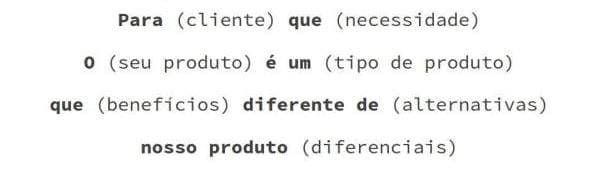
\includegraphics[width=.7\textwidth, scale=6.7]{fig1.jpeg}
\caption{Visão do produto}
\label{fig:typical-figure}
\end{figure}

\subsection{Personas}
Uma persona em UX (User Experience) é uma representação fictícia, porém baseada em dados reais, de um usuário ideal para um produto ou serviço. Ela é criada com o objetivo de ajudar a equipe de UX a compreender melhor as necessidades, objetivos e comportamentos dos usuários.

A criação de uma persona envolve a realização de pesquisas e análises de dados de usuários, como entrevistas, questionários e análise de métricas de uso e comportamento. A partir dessas informações, a equipe de UX pode criar uma persona que representa um usuário típico, retratando suas características demográficas, preferências, comportamentos, necessidades e desafios. A figura 2 ilustra uma persona para um aplicativo de música.

\begin{figure}[ht]
\centering
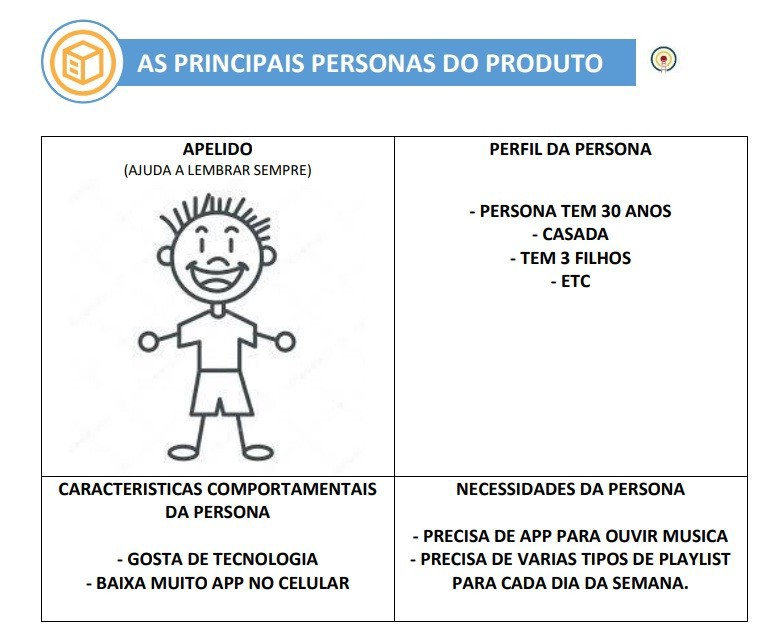
\includegraphics[width=.7\textwidth, scale=6.7]{persona.jpeg}
\caption{Persona}
\label{fig:typical-figure}
\end{figure}

\subsection{Mapa de Empatia}
O mapa de empatia é uma ferramenta visual que destaca as necessidades, desejos, emoções e comportamentos dos clientes ou usuários de um produto ou serviço. Ele coloca o usuário no centro do processo de desenvolvimento, sendo usado no design thinking.
O mapa de empatia é dividido em seis seções que abrangem diferentes aspectos do usuário: o que ele vê, ouve, pensa e sente, fala e faz, suas dores e suas necessidades.
Ao preencher essas seções, obtemos uma visão empática e abrangente do usuário, permitindo criar soluções mais eficazes e centradas nele.
A figura 3 ilustra um exemplo do mapa de empatia.

\begin{figure}[ht]
\centering
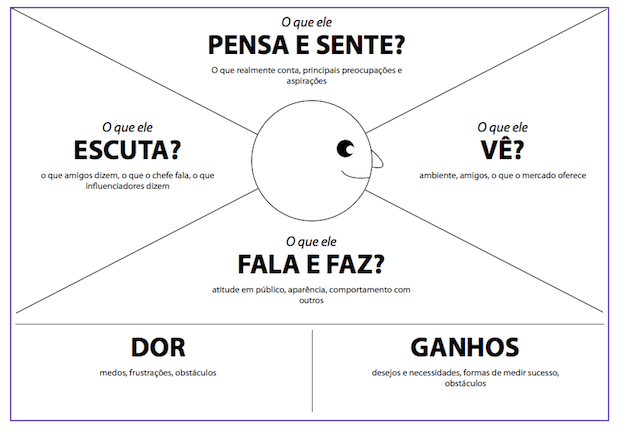
\includegraphics[width=.7\textwidth, scale=6.7]{mapa.png}
\caption{Mapa de empatia}
\label{fig:typical-figure}
\end{figure}

\subsection{Fluxo da Jornada do Usuário}
O fluxo da jornada do usuário é uma representação visual das etapas que um usuário realiza para alcançar um objetivo em um produto ou serviço. É usado em UX para entender a interação do usuário ao longo do tempo, desde a primeira interação até a conclusão da tarefa.
O fluxo da jornada do usuário é criado por meio de diagramas ou wireframes, destacando ações, decisões, feedback e emoções do usuário.

Na figura 4, temos um fluxo básico da jornada do usuário em um aplicativo de entrega de comida, abrangendo desde a pesquisa até a finalização da entrega. O objetivo é oferecer uma experiência simples e conveniente para o usuário, reduzindo possíveis obstáculos e aumentando a satisfação do usuário.

\begin{figure}[ht]
\centering
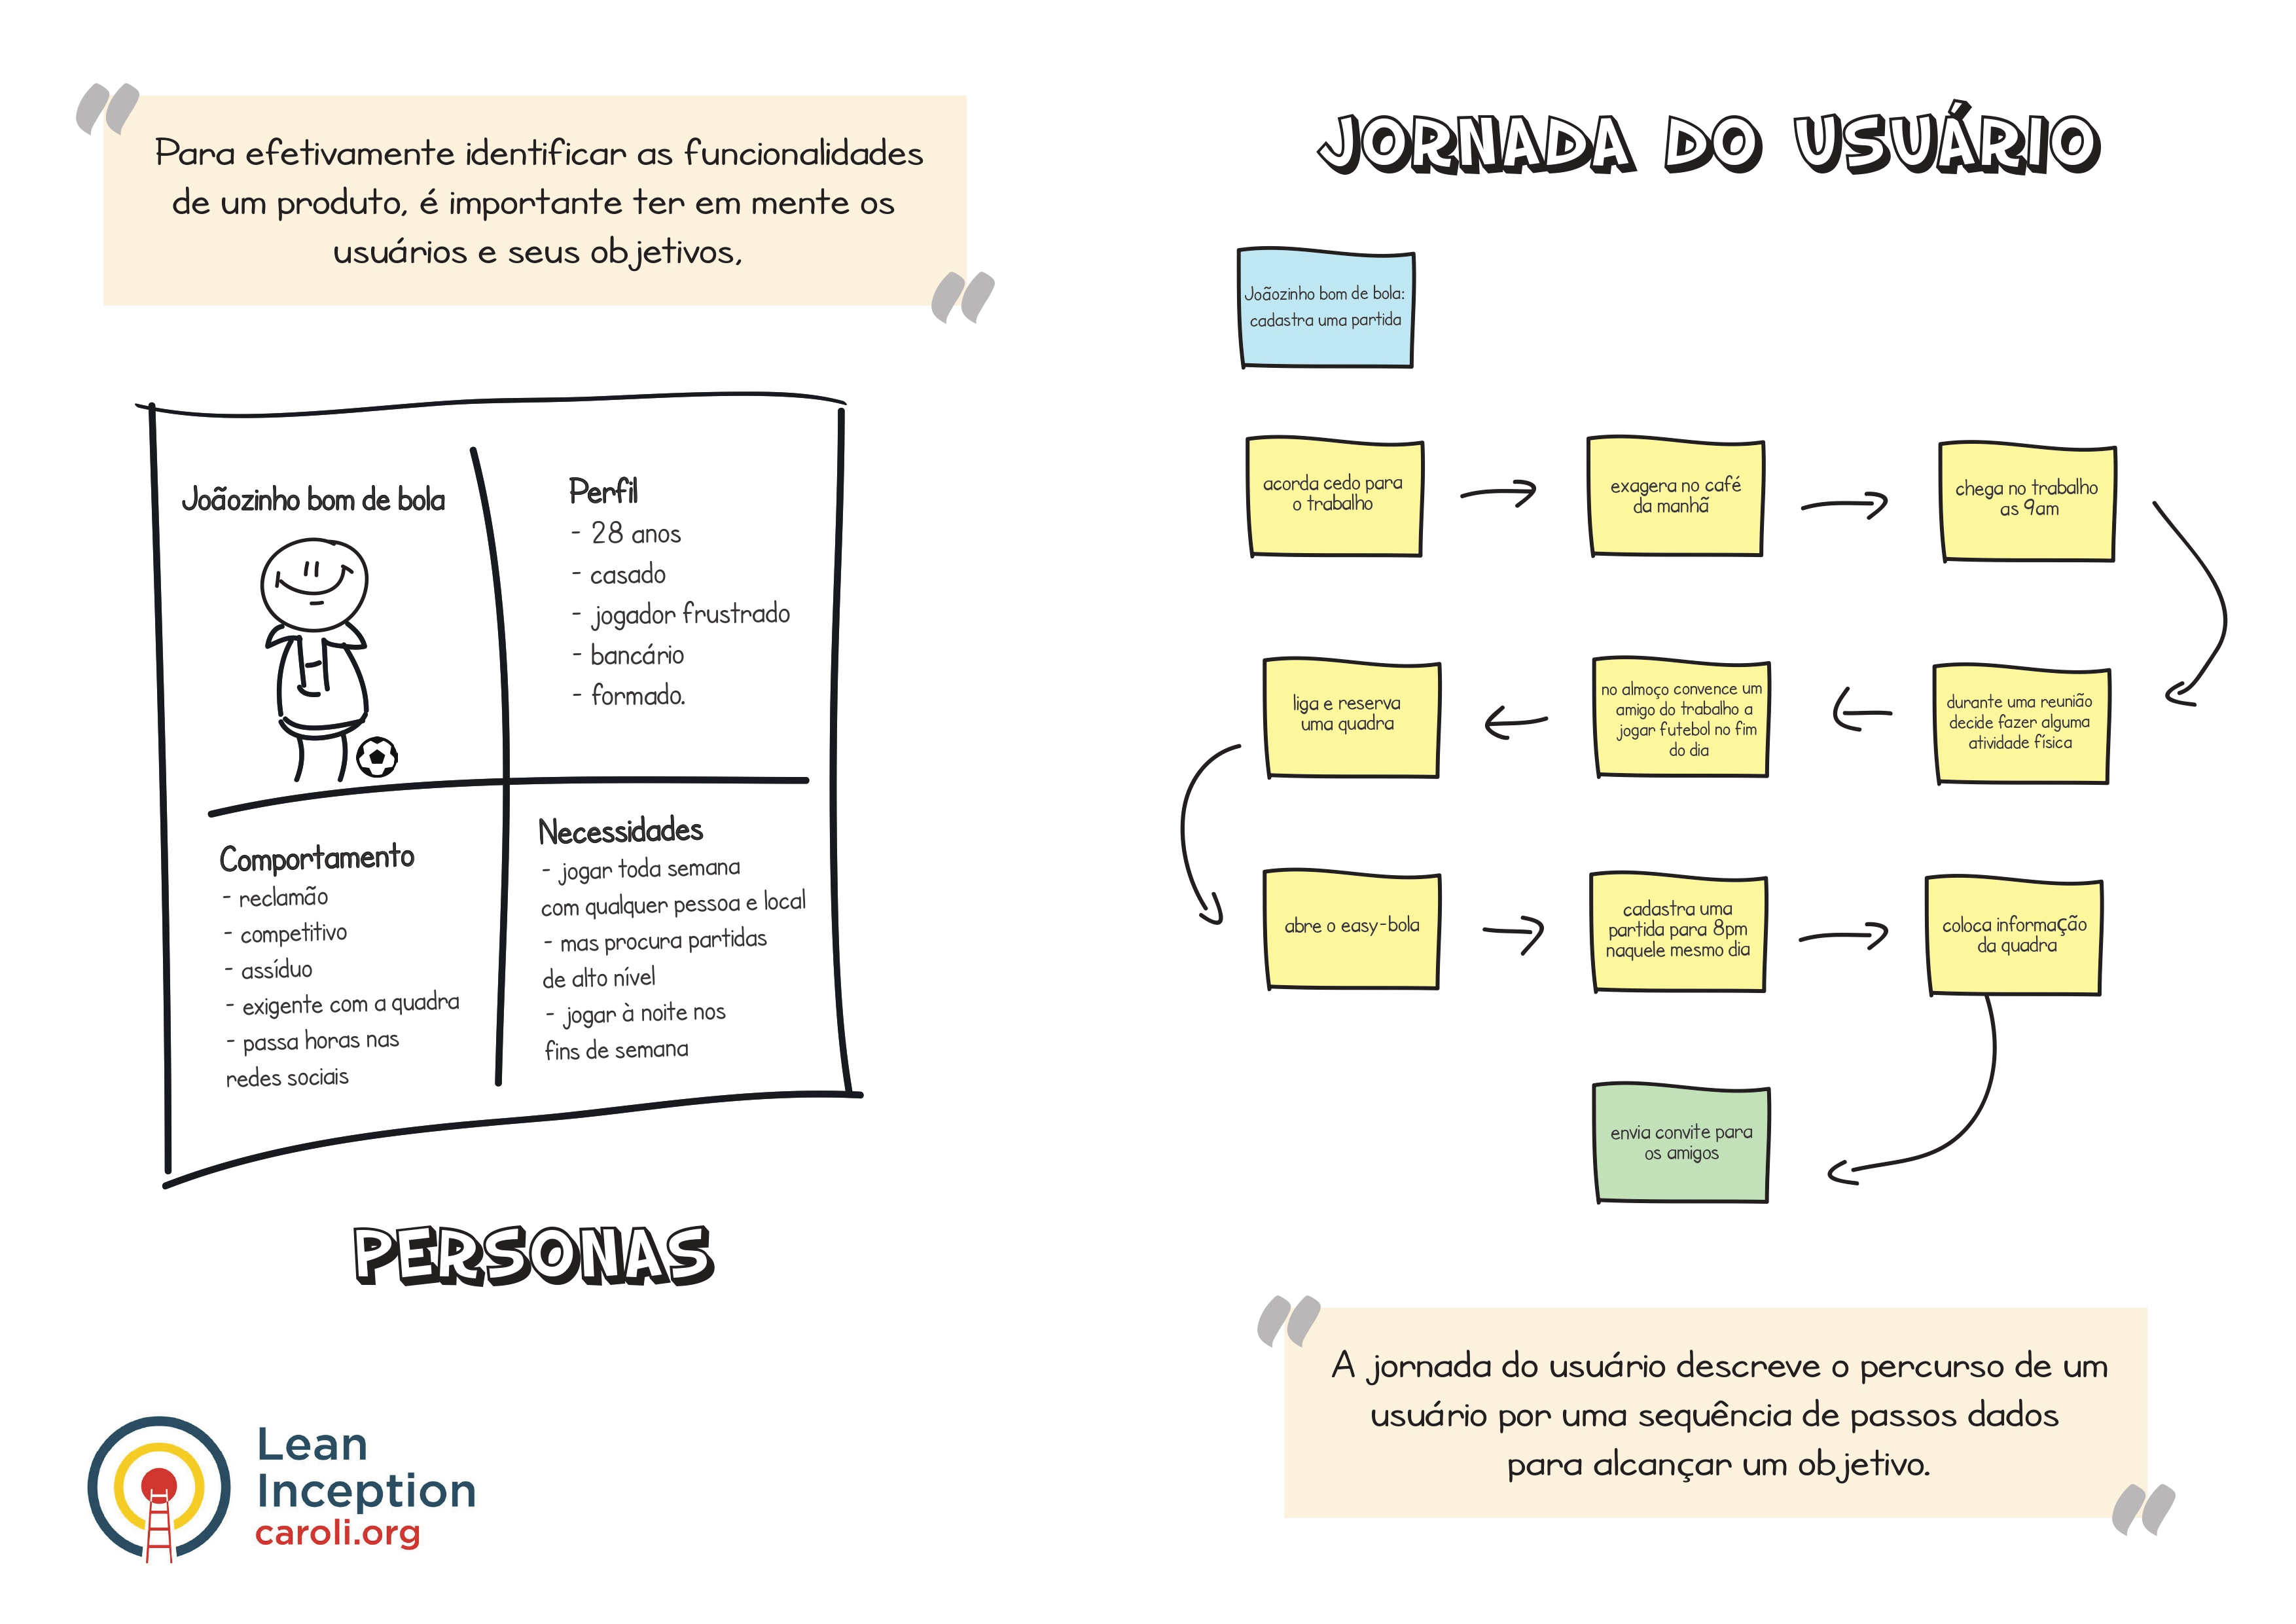
\includegraphics[width=.5\textwidth, scale=6.7]{jornada.jpg}
\caption{Fluxo da jornada do usuário}
\label{fig:typical-figure}
\end{figure}

\subsection{Product Backlog}
Nesta etapa é criado o product backlog que é “Uma sacolinha de
funcionalidades do produto. ”(Aislan Rafael, 2022). Através dele podemos ter uma visão mais focada a utilidade de cada funcionalidade e sua importância para o sistema possibilitando um desenvolvimento mais otimizado. 

O Product Backlog é uma lista priorizada de requisitos, funcionalidades e melhorias necessárias para um produto ou projeto. Ele é constantemente atualizado pelo Product Owner com base no valor de negócio e feedback dos clientes. Durante as reuniões de planejamento do sprint, a equipe seleciona os itens do backlog para trabalhar no próximo ciclo de desenvolvimento. Isso permite um desenvolvimento incremental e adaptativo do produto. A figura 5 ilustra um template para listar o product backlog.

\begin{figure}[H]
\centering
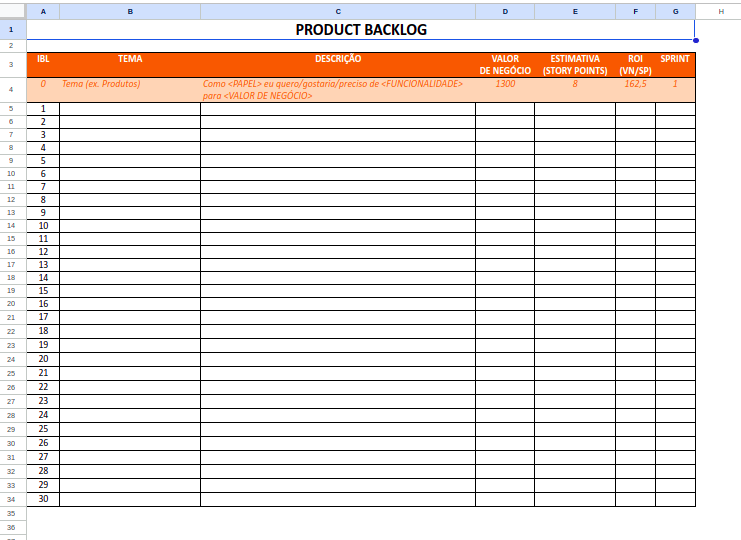
\includegraphics[width=.8\textwidth]{product.png}
\caption{Template do product backlog}
\label{fig:typical-figure}
\end{figure}

\subsection{Rabisco Frame}
O wireframe de baixa fidelidade, também conhecido como rabisco frame, é uma representação visual simplificada de um site ou aplicativo. Ele é usado para planejar a estrutura e o layout do projeto antes do desenvolvimento. Os wireframes de baixa fidelidade são compostos por formas básicas e texto, enfocando a funcionalidade e a experiência do usuário. São rápidos de criar e permitem receber feedback dos stakeholders e da equipe de desenvolvimento em estágios iniciais do projeto. A figura 6 e 7 ilustram um exemplo do rabisco frame. 
\begin{figure}[H]
\centering
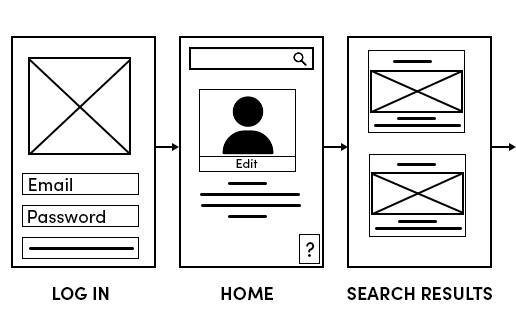
\includegraphics[width=.8\textwidth]{frame1.png}
\caption{Exemplo de um rabisco frame}
\label{fig:typical-figure}
\end{figure}

\begin{figure}[H]
\centering
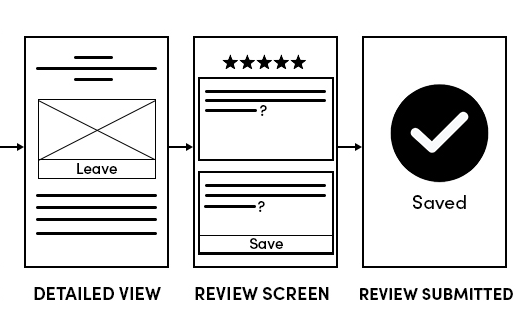
\includegraphics[width=.8\textwidth]{frame2.png}
\caption{Exemplo de um rabisco frame}
\label{fig:typical-figure}
\end{figure}

\section{Conhecendo o sistema}
Neste capítulo serão apresentados as telas e as funcionalidades do sistema
web ou aplicativo.

\subsection{Tecnologias utilizadas}
Neste tópico, fornecemos informações relevantes sobre as ferramentas, linguagens de programação, bibliotecas e frameworks utilizados no desenvolvimento do software em questão. Essas escolhas tecnológicas desempenham um papel fundamental no funcionamento e desempenho do software, e sua compreensão é essencial para uma visão completa do projeto. 

\subsection{Protótipo de telas}
Nesta seção, incluímos imagens das telas do protótipo de software. Um protótipo de software é uma versão preliminar e simplificada do software em desenvolvimento. Ele é criado para testar e validar conceitos, funcionalidades e fluxos de interação antes do desenvolvimento completo. O objetivo principal é obter feedback dos usuários para melhorar o design e a usabilidade. Os protótipos podem variar em fidelidade, desde simples esquemas até representações visuais mais próximas do produto final. A escolha do tipo de protótipo depende dos objetivos e estágio do desenvolvimento do software.

\section{Avaliação}
Nesta seção, serão apresentados os testes de infraestrutura e usabilidade realizados, bem como os resultados obtidos, visando assegurar a confiabilidade, usabilidade e integridade do sistema.

\subsection{Teste de desempenho}
O teste de desempenho avalia o desempenho, estabilidade e escalabilidade de um sistema em condições de carga e estresse. Simula situações reais com muitos usuários ou carga intensiva, analisando o tempo de resposta, taxa de transferência, capacidade de processamento e utilização de recursos. Identificando gargalos e pontos fracos, o teste permite otimizar o sistema, ajustar configurações e melhorar a experiência do usuário. Existem várias ferramentas gratuitas disponíveis para realizar testes de desempenho. Aqui estão alguns exemplos:
\begin{itemize}
   \item Page Speed Insights (O Google PageSpeed: É
uma família de ferramentas do Google Inc, projetada para ajudar na otimização do
desempenho de um site), com esta ferramenta é possível identificar problemas de
codificação, usabilidade, carregamento de páginas e renderização das páginas para
dispositivos de telas diferentes. 
\item Apache JMeter: É uma ferramenta de teste de carga e desempenho amplamente utilizada. Permite simular diferentes cargas de trabalho, medir o desempenho de servidores web, aplicativos e serviços, além de oferecer recursos avançados de relatórios e análise
 \end{itemize}
 
\subsection{Teste de usabilidade}
O teste de usabilidade avalia a facilidade de uso e a experiência do usuário em um produto. Os usuários realizam tarefas enquanto são observados por especialistas. Os resultados identificam problemas e ajudam a melhorar o design e a interação. O teste de usabilidade pode ser realizado seguindo algumas etapas básicas:
\begin{itemize}
   \item Defina os objetivos: Determine quais aspectos do produto você deseja avaliar e quais perguntas deseja responder por meio do teste de usabilidade.
   \item  Identifique o público-alvo: Selecione os usuários que representam o público-alvo do produto. Eles devem ter características que reflitam os usuários reais do produto.
    \item Crie cenários de teste: Desenvolva tarefas ou cenários realistas que os usuários devem realizar durante o teste. Essas tarefas devem abranger os principais recursos e funcionalidades do produto.
    \item Execute o teste: Peça aos usuários selecionados que realizem as tarefas definidas enquanto são observados. Encoraje-os a pensar em voz alta e expressar suas opiniões e dificuldades durante o processo.
    \item Colete feedback e observe: Registre os comentários, observações e comportamentos dos usuários durante o teste. Observe suas ações, reações e expressões faciais para obter insights adicionais.
    \item Analise os resultados: Revise os dados coletados e identifique os padrões, problemas de usabilidade e oportunidades de melhoria. Priorize as áreas que necessitam de ajustes.
\end{itemize}
\subsection{Resultados}
Ao apresentar os resultados obtidos com os testes de usabilidade, é importante destacar os principais insights e descobertas que foram identificados. Aqui estão algumas informações que podem ser abordadas:
\begin{itemize}
    \item Problemas de usabilidade: Descreva os principais problemas ou dificuldades encontrados pelos usuários durante o teste. Isso pode incluir problemas de navegação, falta de clareza nas instruções, confusão de layout, dificuldade em encontrar informações ou executar tarefas específicas. Forneça exemplos concretos e ilustrativos desses problemas.
    \item Feedback dos usuários: Apresente os comentários, opiniões e sugestões dos usuários durante o teste. 
    \item Ações corretivas tomadas: Descreva as medidas corretivas que foram adotadas com base nos resultados dos testes de usabilidade.
\end{itemize}
\section{Considerações Finais}
Nesta seção, apresentaremos um resumo dos principais pontos do relatório, reafirmando o problema identificado, a solução proposta e discutindo as implicações do trabalho. Além disso, sugeriremos possíveis direções para futuros desenvolvimentos. 

\bibliographystyle{sbc}
\bibliography{sbc-template}
\end{document}
